% Source: checkpoints/ablations/no-rmsnorm/train.log, first 1,000 completed updates.
% Training points are unsmoothed minibatch losses; validation uses fixed windows.
\documentclass[tikz,border=4pt]{standalone}
\usepackage[T1]{fontenc}
\usepackage{pgfplots}
\pgfplotsset{compat=1.18}
\begin{document}
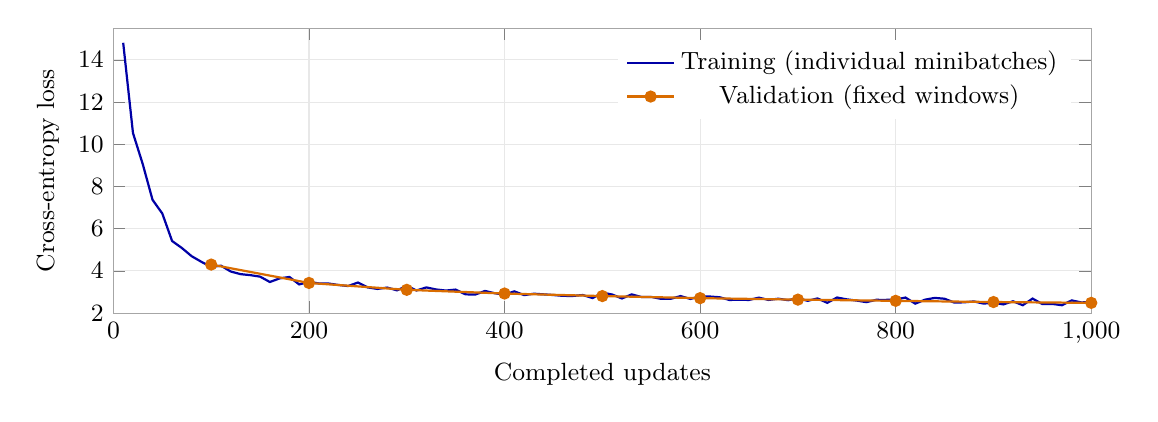
\begin{tikzpicture}
\begin{axis}[
 width=14cm,height=5.2cm,
 xlabel={Completed updates},ylabel={Cross-entropy loss},
 xmin=0,xmax=1000,ymin=2,ymax=15.5,
 xtick={0,200,400,600,800,1000},scaled x ticks=false,
 ytick={2,4,6,8,10,12,14},
 grid=major,grid style={gray!18},
 axis line style={gray!70},tick label style={font=\small},
 label style={font=\small},
 legend style={at={(0.98,0.96)},anchor=north east,font=\small,draw=none,fill=white},
]
\addplot[blue!65!black,thick,no marks] coordinates {(10,14.8097) (20,10.5363) (30,9.0612) (40,7.371) (50,6.7213) (60,5.419) (70,5.0863) (80,4.6985) (90,4.4307) (100,4.1934) (110,4.2472) (120,3.9728) (130,3.8481) (140,3.8011) (150,3.7296) (160,3.4759) (170,3.6465) (180,3.7141) (190,3.3607) (200,3.4848) (210,3.4079) (220,3.4038) (230,3.3351) (240,3.2834) (250,3.4496) (260,3.2187) (270,3.1481) (280,3.2109) (290,3.0801) (300,3.2894) (310,3.075) (320,3.2191) (330,3.1211) (340,3.0696) (350,3.1157) (360,2.891) (370,2.8803) (380,3.0508) (390,2.9435) (400,2.8791) (410,3.0308) (420,2.856) (430,2.9203) (440,2.89) (450,2.8577) (460,2.8181) (470,2.8155) (480,2.858) (490,2.7146) (500,2.9693) (510,2.8837) (520,2.6961) (530,2.8886) (540,2.7645) (550,2.7685) (560,2.6781) (570,2.6803) (580,2.8083) (590,2.6731) (600,2.7918) (610,2.7863) (620,2.7529) (630,2.6235) (640,2.6388) (650,2.6244) (660,2.7343) (670,2.6259) (680,2.6834) (690,2.6141) (700,2.7099) (710,2.583) (720,2.6975) (730,2.4886) (740,2.7399) (750,2.6531) (760,2.5965) (770,2.5212) (780,2.6299) (790,2.6284) (800,2.6478) (810,2.7382) (820,2.4504) (830,2.6381) (840,2.7221) (850,2.6823) (860,2.4991) (870,2.5128) (880,2.5536) (890,2.4522) (900,2.4966) (910,2.4138) (920,2.5621) (930,2.3754) (940,2.6896) (950,2.4294) (960,2.4382) (970,2.3756) (980,2.6036) (990,2.5057) (1000,2.5383)};
\addlegendentry{Training (individual minibatches)}
\addplot[orange!85!black,thick,mark=*,mark size=1.8pt] coordinates {(100,4.3012) (200,3.4302) (300,3.105) (400,2.9291) (500,2.8088) (600,2.7106) (700,2.6405) (800,2.5834) (900,2.5264) (1000,2.4872)};
\addlegendentry{Validation (fixed windows)}
\end{axis}
\end{tikzpicture}
\end{document}
